\documentclass[a4paper, 11pt]{article}

% Compiler avec XeLaTeX !!

\usepackage{amsmath}
\usepackage{amssymb}
\usepackage{stmaryrd}

\usepackage{unicode-math}
\usepackage{polyglossia}
\setmainlanguage{french}
\usepackage{csquotes} % guillemets

% Changer choix de police ? Palatino est plus assez hipster pour moi
\setmainfont[Mapping=tex-text]{TeX Gyre Pagella}
\setmathfont{Asana-Math.otf}

\usepackage{fullpage} % pour faire tenir les règles sur la page

% TikZ for proof nets, graphs...
\usepackage{tikz}
\usetikzlibrary{shapes,arrows}

%% Configuration propre à la logique linéaire

% Arbres de preuves de séquents
\usepackage{bussproofs}

% Opérateurs propres à la logique linéaire
% Mieux que le package cmll car ça utilise la bonne police avec unicode
% tenseur = \otimes, ou additif = \oplus
\newcommand{\avec}{\mathbin{\&}}
\newcommand{\parr}{\mathbin{⅋}}
\newcommand{\ofcourse}{\mathord{!}}
\newcommand{\whynot}{\mathord{?}}

\begin{document}

\title{Logique linéaire et paradigmes logiques du calcul}
\author{Cours MPRI 2.1}
\date{2013--2014}

\maketitle

% Pour rendre les tableaux de règles avec tabular plus agréables.
\renewcommand{\arraystretch}{2}



BROUILLON TRES PRELIMINAIRE.

Synopsis du cours pompé sur la page web :

\enquote{Une analyse fine des calculs de séquents classiques et intuitionnistes permet de concevoir des logiques plus adaptées aux problèmes de l'informatique et de dévélopper, grâce à la correspondance de Curry-Howard des formalismes intermédiaires entre le $\lambda$-calcul et les vrais langages de programmation.

Ce cours a pour but de donner une vision d'ensemble des motivations et des applications d'une de ces logiques, la Logique Linéaire, qui permet une analyse plus fine des processus de démonstration et de calcul, et d'introduire les notions de base des calculs intermédiaires les plus connus. On montrera dans le cours comment ces deux approches se rejoignent, à travers des interprétations calculatoires adaptées.

Ce cours dédie une attention toute particulière aux aspects syntaxiques et calculatoires des formalismes logiques.}


Pour la sémantique, voir le cours \enquote{Modèles de la programmation}, notamment la partie de P.A Melliès.

Intervenants en 2013--2014 : Roberto di Cosmo, Delia Kesner\ldots ajouter calendrier ?


Références :
\begin{itemize}
\item The Linear Logic Primer (Vincent Danos et Roberto Di Cosmo)
\item Proof and Types (Jean-Yves Girard, traduit par Yves Lafont et Paul Taylor)
\item more to come\ldots
\end{itemize}

Ajouter une liste d'articles ?

Les titres des sections ne sont pas fixés. Les suggestions sont bienvenues.

Dans la hiérarchie de la table des matières, on a
\begin{itemize}
\item Section $\simeq$ intervenant (ou thème)
\item Sous-section $\simeq$ Séance de cours
\item Sous-sous-section $\simeq$ partie au sein d'une séance
\end{itemize}

\newpage

\tableofcontents

\newpage

\section{Introduction à la logique linéaire}

\subsection{Du calcul des séquents à la logique linéaire}

L'histoire du programme de Hilbert et de son échec (théorème d'incomplétude) est bien connue. Vers la même période où Gödel montre l'impossibilité d'une preuve de cohérence de $PA$ (l'arithmétique de Peano) dans lui-même, Gentzen parvient à montrer que $PA$ est cohérente par une induction jusqu'à l'ordinal $\varepsilon_0$. Pour cela, il introduit des systèmes de preuves, la \emph{déduction naturelle} et le \emph{calcul des séquents}, et ramène l'absence de contradiction du système à la terminaison d'une procédure d'\emph{élimination des coupures} sur les preuves, s'approchant ainsi du rêve finitiste hilbertien. Contrairement aux systèmes dits \enquote{à la Hilbert}, ceux de Gentzen contiennent peu d'axiomes, mais beaucoup de règles de déduction.

Les sytèmes de preuves que nous allons étudier sont constitués de règles formelles permettant de \emph{dériver} des \emph{jugements}. Un jugement est de la forme $\Gamma \vdash \Delta$, où $\Gamma$ et $\Delta$ sont des \emph{séquents}, c'est-à-dire des listes de formules de la forme $A_1, \ldots, A_n$. (Le symbole $\vdash$ s'appelle \enquote{turnstile} et est prononcé \enquote{thèse} en français.) $\Gamma \vdash \Delta$ signifie informellement \enquote{à partir des hypothèses $\Gamma$, on déduit les conclusions $\Delta$}, sachant que l'interprétation de la virgule et du turnstile sont à préciser en fonction du système.

Les règles du calcul sont écrites sous la forme
\begin{prooftree}
\AxiomC{$A_1$}
\AxiomC{$A_2$}
\AxiomC{\ldots}
\AxiomC{$A_n$}
\RightLabel{\mbox{(nom de la règle)}}
\QuaternaryInfC{$B$}
\end{prooftree}
où les $A_i$ et $B$ sont des jugements, la barre verticale signifiant \enquote{si les jugements $A_i$ sont valides, alors $B$ l'est}. En construisant un arbre dont les noeuds sont des applications de ces règles, on obtient une \emph{preuve} dans le système (aussi appelée dérivation).

Commençons par le calcul des séquents qui se décline en variantes classique (LK) et intuitionniste (LJ).

\subsubsection{Logique classique : le système LK de Gentzen}

En LK, $A_1, \ldots, A_n \vdash B_1, \ldots, B_m$ signifie \enquote{$A_1$ et $A_2$ \ldots et $A_n$ prouve $B_1$ ou $B_2$ \ldots ou $B_m$}, ou encore \enquote{si tous les $A_i$ sont vrais, l'un des $B_j$ sera vrai}. La virgule n'a pas la même signification des 2 côtés du turnstile !

Voici les règles du système LK :

\paragraph{Axiome} L'axiome est la règle permettant d'introduire une prémisse présente dans la liste des hypothèse. C'est la seule règle sans \enquote{hypothèse}\footnote{il faudrait trouver un meilleur nom pour distinguer avec les hypothèses d'un jugement} : les feuilles d'un arbres de preuve sont obligatoirement des axiomes. \\
Elle s'écrit
\begin{prooftree}
\AxiomC{}
\RightLabel{(Ax)}
\UnaryInfC{$\Gamma, A \vdash A, \Delta$}
\end{prooftree}
Interprétation : \ldots

\paragraph{Coupure} Cette règle est en même temps essentielle et inutile (on verra pourquoi après). Elle correspond à l'emploi, dans la preuve d'un théorème, d'un lemme préalablement prouvé.
Elle s'écrit :
\begin{prooftree}
\AxiomC{$\Gamma \vdash A, \Delta$}
\AxiomC{$\Gamma', A \vdash \Delta'$}
\RightLabel{(Cut)}
\BinaryInfC{$\Gamma, \Gamma' \vdash \Delta, \Delta'$}
\end{prooftree}
blabla pour préciser l'interprétation

\paragraph{Règles structurelles} La flemme d'écrire ça\ldots échange + contraction + affaiblissement avec versions à gauche et à droite. Dans mes notes de cours, j'ai :
\begin{itemize}
\item contraction : l'immuabilité de la vérité permet d'utiliser des hypothèses plusieurs fois
\item affaiblissement : élargir les hypothèses ; (permet de faire des manips sur le système lui-même ??)
\end{itemize}
Ces règles peuvent paraître anodines, elles semblent tomber sous le sens. Pourtant, elles vont se révéler très importante.

\paragraph{Règles logiques} Règles permettant l'introduction des connecteurs, manifestant ainsi dans la syntaxe des formules la structure du système logique. Pour avoir un équivalent des règles d'élimination de la déduction naturelle, utiliser intro + coupure.
Copier depuis en bas.
2 présentations, mult et add. équivalence : emploie les règles structurelles.

\begin{prooftree}
\AxiomC{$\Gamma, A \vdash \Delta$}
\UnaryInfC{$\Gamma \vdash \neg A, \Delta$}  
\end{prooftree}
\begin{prooftree}
\AxiomC{$\Gamma \vdash A, \Delta$}
\UnaryInfC{$\Gamma, \neg A \vdash \Delta$}  
\end{prooftree}

\paragraph{Quantification} Pour faire de la logique du 1er ordre.

\paragraph{} Comme exemple, voici une preuve du tiers exclu sans hypothèse en LK :
\begin{prooftree}
  \AxiomC{}
  \RightLabel{(Ax)}
  \UnaryInfC{$A \vdash A$}
  \UnaryInfC{$\vdash A, \neg A$}
  \RightLabel{($\lor_R$)}
  \UnaryInfC{$\vdash A \lor \neg A$}
\end{prooftree}

\paragraph{Jolies propriétés du système LK} En voici quelques-unes simples :
\begin{itemize}
\item Il y a une symétrie dans le calcul entre les 2 côtés du $\vdash$, en passant entre les 2 par la négation. La symétrie se traduit aussi par la dualité entre les connecteurs $\land$ et $\lor$, dont les règles se déduisent en échangeant gauche et droite.
\item La négation est une involution, i.e. $\neg\neg A \equiv A$.
\item Cette logique admet des modèles simples, les algèbres de Boole. Les formules valides en algèbre booléenne sont exactement celles démontrables en LK.
\end{itemize}

La propriété la plus importante est la \emph{propriété de la sous-formule}, vérifiée par les preuves dites \emph{sans coupure}, celles qui ne font pas appel à la règle de coupure. Cette propriété est que la démonstration ne fait pas intervenir de formules \enquote{sorties de nulle part} : les formules intermédiaires de l'arbre de preuve sont contenues dans la conclusion.

Ce qui rend d'autant plus pertinent cette propriété est le théorème d'\emph{élimination des coupures} (ou Hauptsatz\footnote{\enquote{théorème fondamental} en allemand} de Gentzen) :
\[ \Gamma \vdash_{\mathrm{LK}} \Delta \Leftrightarrow 
   \Gamma \vdash_{\mathrm{LK} \setminus \mathrm{Cut}} \Delta \]
Autrement dit, tout jugement dérivable en LK admet une preuve sans coupure.

Ce théorème permet de prouver la cohérence du système, c'est-à-dire l'absence de contradiction, qu'on pourrait formuler $\not\vdash A \land \neg A$. Une preuve sans coupure de $\vdash A \land \neg A$ devrait se terminer par
\begin{prooftree}
  \AxiomC{\vdots}
  \UnaryInfC{$\vdash A$}
  \AxiomC{\vdots}
  \UnaryInfC{$A \vdash$}
  \UnaryInfC{$\vdash \neg A$}
  \BinaryInfC{$\vdash A \land \neg A$}
\end{prooftree}
or $\vdash A$ et $A \vdash$ ne peuvent être prouvés sans coupure.

\paragraph{LK est non constructive} En LK, on peut obtenir des preuves d'existence sans pouvoir obtenir un témoin de cette existence. En voici un exemple célèbre, le \enquote{drinker paradox}\footnote{le nom est dû à l'interprétation suivante en langue naturelle : dans un bar (non vide), il y a quelqu'un tel que si cette personne boit, tout le monde boit.}, qui consiste en la formule : $\exists x\, (P(x) \Rightarrow \forall y\, P(y))$.

\begin{prooftree}
    \AxiomC{}
    \UnaryInfC{$P(x), P(z) \vdash P(z), \forall y . P(y)$}
    \UnaryInfC{$P(x) \vdash P(z), P(z) \Rightarrow \forall y . P(y)$}
    \UnaryInfC{$P(x) \vdash P(z), \exists x (P(x) \Rightarrow \forall y . P(y))$}
    \UnaryInfC{$P(x) \vdash \forall y . P(y), \exists x. (P(x) \Rightarrow \forall y . P(y))$}
    \UnaryInfC{$\vdash P(x) \Rightarrow \forall y . P(y), \exists x . (P(x) \Rightarrow \forall y . P(y))$}
    \UnaryInfC{$\vdash \exists x . (P(x) \Rightarrow \forall y . P(y)), \exists x (P(y) \Rightarrow \forall y . P(y))$}
    \UnaryInfC{$\vdash \exists x . (P(x) \Rightarrow \forall y . P(y))$}
\end{prooftree}

\emph{Remarque importante :} on a employé de façon cruciale la règle de contraction ; c'est une indication du pouvoir insoupçonné des règles structurelles. (Notez que la contraction permet de passer de $\neg A \vdash A$ à $\vdash A$ : c'est le raisonnement par l'absurde !)

\subsubsection{Logique intuitionniste : le système LJ}

Pour obtenir une logique constructive, on peut procéder à une mutilation brutale des symétries de LK : on va interdire la présence de plusieurs formules à droite, ce qui restreint fortement la flexibilité des règles structurelles et de la manipulation de la négation. La logique obtenue ainsi est nommée LJ, c'est une formalisation de la logique \emph{intuitionniste} (elle est équivalente au système NJ de Prawitz, qui correspond au lambda-calcul typé). En LJ, un jugement est de la forme $\Gamma \vdash A$, où $\Gamma$ est un séquent et $A$ une formule, ou alors de la forme $\Gamma \vdash$.

On obtient bien la constructivité, qui s'exprime par le théorème suivant (\emph{propriété de la disjonction}) : si $\Gamma \vdash A \lor B$, alors $\Gamma \vdash A$ ou $\Gamma \vdash B$. En particulier, $\not\vdash A \lor \neg A$ ; on pourra vérifier que la preuve du tiers exclu plus haut ne marche plus.

Cependant, LJ a de nombreux inconvénients par rapport à LK. Tout d'abord, les modèles de la logique intuitionniste sont bien plus compliqués (modèles de Kripke, etc.). Surtout, on a perdu toute la symétrie : la gauche et la droite du $\vdash$ se comportent différemment, les connecteurs ne sont plus interdéfinissables, et la négation n'est plus involutive. Quel prix à payer !\footnote{Paul-André Melliès considère que l'insistance de la logique linéaire sur la négation involutive est malavisée. Cf. les travaux sur la logique tensorielle.}

Plutôt que de briser la symétrie, on peut s'y prendre en contrôlant les règles structurelles : cette alternative s'appelle la \emph{logique linéaire}.

\subsubsection{Le meilleur des deux mondes : la logique linéaire}

La logique linéaire repose sur une interprétation des formules en termes de \emph{ressources}.
\begin{itemize}
\item En logique classique, $A \Rightarrow B$ signifie simplement \enquote{si $A$, alors $B$}.
\item En logique intuitionniste, on interprète\footnote{Il s'agit de l'interprétation dite de Brower--Heyting--Kolmogorov.} $A \Rightarrow B$ comme une fonction qui prend une preuve de $A$ et renvoie une preuve de $B$. On pourrait voir ça comme une machine qui transforme une machine productrice de $A$ en machine productrice de $B$.
\item En logique linéaire, on a une notion de consommation : on va interpréter l'implication linéaire $A \multimap B$ comme \enquote{je consomme exactement 1 $A$, et je produis exactement 1 $B$}.
\end{itemize}
Selon cette interprétation \enquote{économique}, les règles de contraction et d'affaiblissement sont suspectes (on pourrait faire avec 1 $A$ la même chose qu'avec 2 $A$ ?). On va donc supprimer ces règles en logique linéaire.

En reprenant les règles logiques du système LK, on verra que la logique linéaire restaure la symétrie et la dualité. Quid du tiers exclu ? En fait, en LL, il va y avoir deux connecteurs différents correspondant au \enquote{ou} logique, notés $\parr$ et $\oplus$. Le tiers exclu dépend du \enquote{ou} : on a $\vdash A \parr \neg A$, mais $\not\vdash A \oplus \neg A$ !


\subsection{Le système LL}

Souvenons-nous des deux présentations des règles logiques en LK. En l'absence des règles structurelles, elles ne sont pas équivalentes ; on va donc se retrouver avec 2 jeux de règles, les règles multiplicatives et les règles additives, définissant 2 \enquote{et} et 2 \enquote{ou} différents.

\subsubsection{Règles logiques}

\paragraph{Axiome} S'écrit simplement\AxiomC{} \RightLabel{(Ax)} \UnaryInfC{$A \vdash A$} \DisplayProof \\
Pas de contexte supplémentaire à gauche ou à droite.

\paragraph{Coupure}
\AxiomC{$\Gamma \vdash A, \Delta$}
\AxiomC{$\Gamma', A \vdash \Delta'$}
\RightLabel{(Cut)}
\BinaryInfC{$\Gamma, \Gamma' \vdash \Delta, \Delta'$}
\DisplayProof
: comme en LK

\paragraph{Connecteurs multiplicatifs}

\begin{itemize}
\item Le \enquote{et} multiplicatif est $\otimes$, prononcé \enquote{tenseur}.
\item Le \enquote{ou} multiplicatif est $\parr$,   prononcé \enquote{par}.
\end{itemize}

\begin{tabular}{ l r }

\AxiomC{$\Gamma, A, B, \vdash \Delta$}
\RightLabel{($\otimes$L)}
\UnaryInfC{$\Gamma, A \otimes B \vdash \Delta$}
\DisplayProof

&

\AxiomC{$\Gamma  \vdash A, \Delta$}
\AxiomC{$\Gamma' \vdash B, \Delta'$}
\RightLabel{($\otimes$R)}
\BinaryInfC{$\Gamma, \Gamma' \vdash A \otimes B, \Delta, \Delta'$}
\DisplayProof

\\

\AxiomC{$\Gamma,  A \vdash \Delta$}
\AxiomC{$\Gamma', B \vdash \Delta'$}
\RightLabel{($\parr$L)}
\BinaryInfC{$\Gamma, \Gamma', A \parr B \vdash \Delta, \Delta'$}
\DisplayProof

&

\AxiomC{$\Gamma  \vdash A, B, \Delta$}
\RightLabel{($\parr$R)}
\UnaryInfC{$\Gamma \vdash A \parr B, \Delta$}
\DisplayProof

\end{tabular}


\paragraph{Connecteurs additifs}

\begin{itemize}
\item Le \enquote{et} additif est $\avec$,  prononcé \enquote{avec}.
\item Le \enquote{ou} additif est $\oplus$, prononcé \enquote{plus}.
\end{itemize}

\begin{tabular}{l}

\AxiomC{$\Gamma, A \vdash \Delta$}
\RightLabel{($\avec$L1)}
\UnaryInfC{$\Gamma, A \avec B \vdash \Delta$}
\DisplayProof

\,

\AxiomC{$\Gamma, B \vdash \Delta$}
\RightLabel{($\avec$L2)}
\UnaryInfC{$\Gamma, A \avec B \vdash \Delta$}
\DisplayProof

\qquad

\AxiomC{$\Gamma \vdash A, \Delta$}
\AxiomC{$\Gamma \vdash B, \Delta$}
\RightLabel{($\avec$R)}
\BinaryInfC{$\Gamma \vdash A \avec B, \Delta$}
\DisplayProof

\\

\AxiomC{$\Gamma, A \vdash \Delta$}
\AxiomC{$\Gamma, B \vdash \Delta$}
\RightLabel{($\oplus$L)}
\BinaryInfC{$\Gamma, A \oplus B \vdash \Delta$}
\DisplayProof

\qquad

\AxiomC{$\Gamma \vdash A, \Delta$}
\RightLabel{($\oplus$R1)}
\UnaryInfC{$\Gamma \vdash A \oplus B, \Delta$}
\DisplayProof

\,

\AxiomC{$\Gamma \vdash B, \Delta$}
\RightLabel{($\oplus$R2)}
\UnaryInfC{$\Gamma \vdash A \oplus B, \Delta$}
\DisplayProof

\end{tabular}

\paragraph{La négation} Elle ne change pas par rapport à LK : elle marque le passage entre les deux côtés du $\vdash$, et est involutive.

\paragraph{L'implication linéaire} Notée $\multimap$ (lollipop), elle est donnée par les mêmes règles que l'implication classique. Elle est multiplicative. On a $A \multimap B \equiv \neg A \parr B$.

\AxiomC{$\Gamma \vdash A, \Delta$}
\AxiomC{$\Gamma', B \vdash \Delta'$}
\RightLabel{($\multimap$L)}
\BinaryInfC{$\Gamma, \Gamma', A \multimap B \vdash \Delta, \Delta'$}
\DisplayProof
\quad
\AxiomC{$\Gamma, A \vdash B, \Delta$}
\RightLabel{($\parr$R)}
\UnaryInfC{$\Gamma \vdash A \multimap B, \Delta$}
\DisplayProof


\subsubsection{Modalités exponentielles et règles structurelles}

De la même façon qu'il est possible d'encoder la logique classique dans la logique intuitionniste par \enquote{double-negation translation}, on voudrait pouvoir plonger LJ dans LL. Pour cela, il faudrait être capable de parler de ressources qui ne coûtent rien, telles les propositions vraies de la logique intuitionniste, qui restent valables après utilisation. On va donc réintroduire la contraction et l'affaiblissement, mais de manière contrôlée, en signalant leur champ d'applicabilité par des \emph{modalités} :
\begin{itemize}
\item $\ofcourse A$ : \enquote{autant de $A$ qu'on veut}, prononcé \enquote{bien sûr $A$}.
\item $\whynot A$ : \enquote{un $A$ jetable}, prononcé \enquote{pourquoi pas $A$}.
\end{itemize}
Bien entendu, $\ofcourse$ et $\whynot$ seront duaux. Grâce à ces modalités, on pourra exprimer l'implication intuitionniste $A \Rightarrow B = \ofcourse A \multimap B$, qui sera la traduction de l'implication de LJ.

% Noms des règles repris depuis l'article sur plato.stanford.edu

\paragraph{Contraction}
\AxiomC{$\Gamma, \ofcourse A, \ofcourse A \vdash\Delta$}
\RightLabel{($\ofcourse$C)}
\UnaryInfC{$\Gamma, \ofcourse A \vdash \Delta$}
\DisplayProof
\;
\AxiomC{$\Gamma \vdash \whynot A, \whynot A, \Delta$}
\RightLabel{($\whynot$C)}
\UnaryInfC{$\Gamma \vdash \whynot A, \Delta$}
\DisplayProof


\paragraph{Affaiblissement} 
\AxiomC{$\Gamma \vdash\Delta$}
\RightLabel{($\ofcourse$W)}
\UnaryInfC{$\Gamma, \ofcourse A \vdash \Delta$}
\DisplayProof
\;
\AxiomC{$\Gamma \vdash \Delta$}
\RightLabel{($\whynot$W)}
\UnaryInfC{$\Gamma \vdash \whynot A, \Delta$}
\DisplayProof

\paragraph{Règles d'introduction}

\begin{tabular}{ l r }

\AxiomC{$\Gamma, A \vdash \Delta$}
\RightLabel{($\ofcourse$L)}
\UnaryInfC{$\Gamma, \ofcourse A \vdash \Delta$}
\DisplayProof

&

\AxiomC{$\ofcourse \Gamma \vdash \whynot \Delta, A$}
\RightLabel{($\ofcourse$R)}
\UnaryInfC{$\ofcourse \Gamma \vdash \whynot \Delta, \ofcourse A$}
\DisplayProof

\\

\AxiomC{$\ofcourse \Gamma, A \vdash \whynot \Delta$}
\RightLabel{($\whynot$L)}
\UnaryInfC{$\ofcourse \Gamma, \whynot A \vdash \whynot \Delta$}
\DisplayProof

&

\AxiomC{$\Gamma  \vdash A, \Delta$}
\RightLabel{(?R)}
\UnaryInfC{$\Gamma, \vdash \whynot A, \Delta$}
\DisplayProof

\end{tabular}

(Abréviation : si $\Gamma = A_1,\ldots,A_n$, $\ofcourse \Gamma = \ofcourse A_1, \ldots, \ofcourse A_n$.)

Les règles d'introduction sont aussi appelées :
\begin{itemize}
\item \emph{déréliction} pour $\ofcourse$L et $\whynot$R
\item \emph{promotion} pour $\whynot$L et $\ofcourse$R
\end{itemize}

\subsubsection{Interprétation des connecteurs}

Voilà un exemple qui permet de saisir les différences entre les connecteurs de la logique linéaire :
un menu dans un restaurant.

{ \centering
Menu à 75 Frs

Entrée

Quiche lorraine

ou

Saumon fumé

et

Plat

Pot-au-feu

ou

Filet de canard

et Fruit

selon saison (banane ou raisin ou oranges ou ananas)

ou

Dessert au choix (mistère, glace, tarte aux pommes)

}

Traduit en logique linéaire, cela donne :

$$75 FF^{\bot} \parr ((Q \avec S) \otimes (P \avec F) \otimes (B \oplus R \oplus O \oplus A) \otimes (M \avec G \avec T))$$ 

Pour résumer :
\begin{itemize}
    \item $A \otimes B$ nous permet d'obtenir $A$ et $B$ simultanément
    \item $A \avec B$ nous permet d'avoir soit $A$ soit $B$, et c'est nous qui choisissons lequel on obtient
    \item $A \oplus B$ nous permet d'avoir soit $A$ soit $B$, mais on ne peut pas décider lequel on va obtenir
    \item $A \parr B$ nous permet d'avoir $B$ si on donne un truc qui consomme $A$, c'est à dire $A^{\bot}$, et vice-versa
    \item $A \multimap B$ nous permet de transformer un $A$ en $B$
\end{itemize}

Le \enquote{par} est plus difficile à expliquer avec du langage courant. On peut le voir comme une version symétrisée de l'implication : si j'ai $A \parr B$, j'aurai $A$ si j'ai déjà $B^\perp$, et j'aurai $B$ si j'ai déjà $A^\perp$. $A^\perp \multimap B \equiv A \parr B \equiv B \parr A \equiv B^\perp \multimap A$ : la commutativité de $\parr$ correspond à la contraposition.

\subsubsection{Fragments de la logique linéaire}

\begin{itemize}
\item MLL : logique linéaire multiplicative, ne contient que les connecteurs $\otimes$ et $\parr$
\item MALL : LL sans exponentielles
\item MELL : LL sans additifs
\end{itemize}
Tous ces fragments admettent l'élimination des coupures.

Résultats de complexité pour la dérivabilité :
\begin{itemize}
\item dans MLL : NP-complet
\item dans MALL : PSPACE-complet
\item dans LL : indécidable %indédicable. Hello google.
\end{itemize}
%MELL : Problème ouvert

\subsubsection{Catégoricité des connecteurs}

(sans lien avec la théorie des catégories)

Un connecteur est dit \emph{catégorique} lorsqu'il est pleinement défini par ses règles d'introduction. C'est le cas des tous les connecteurs en MALL. Voici un exemple :

\paragraph{Exercice :} on définit le connecteur $\ast$ par
\AxiomC{$\Gamma,  A \vdash \Delta$}
\AxiomC{$\Gamma', B \vdash \Delta'$}
\BinaryInfC{$\Gamma, \Gamma', A \ast B \vdash \Delta, \Delta'$}
\DisplayProof
\;
\AxiomC{$\Gamma  \vdash A, B, \Delta$}
\UnaryInfC{$\Gamma, \vdash A \ast B, \Delta$}
\DisplayProof \\
Montrer que $\ast$ et $\parr$ sont équivalents.

\paragraph{} Par contre, la catégoricité n'est pas vérifiée dans certaines logiques modales, par exemple LTL\footnote{Linear Temporal Logic.}. (c'est vrai ça ? les présentations de LTL n'emploient pas des règles d'inférences pour définir les connecteurs, de toute façon...)

(exponentielles : catégoriques avec la bonne présentation ?)

Une propriété formelle qui distingue les exponentielles des connecteurs MALL, c'est la présence de contraintes imposées sur le contexte dans les règles d'inférence. Par exemple, dans l'introduction du $\ofcourse$, le contexte à gauche doit être de la forme $\ofcourse \Gamma$, et le contexte à droite doit s'écrire $\whynot \Delta$.

\subsubsection{Présentation asymétrique de LL}

En exploitant la symétrie, on va transformer les règles pour se ramener à un système où les séquents n'apparaissent qu'à droite. Par dualité, la moitié des règles est redondante, on peut ne garder que les règles droites. Puis on transforme $\Gamma \vdash \Delta$ en $\vdash \neg \Gamma, \Delta$ ; souvent, on peut purement et simplement effacer $\Gamma$.

On se retrouve alors avec un problème avec la négation : comment convertir l'introduction de la négation ? Si on passe tout à droite :
\begin{itemize}
\item soit on obtient
  \AxiomC{$\vdash \neg A, \Delta$}
  \UnaryInfC{$\vdash \neg A, \Delta$}
  \DisplayProof
  ce qui est une profonde trivialité
\item soit on obtient
  \AxiomC{$\vdash A, \Delta$}
  \UnaryInfC{$\vdash \neg \neg A, \Delta$}
  \DisplayProof
  qui ne permet d'introduire que des doubles négations : \\c'est pas terrible
\end{itemize}
Idée géniale : ne pas considérer la négation comme un connecteur, mais comme une opération !

On va prendre pour univers des atomes un ensemble infini muni d'une involution $x \mapsto x^\perp$. La négation sera alors définie par induction structurelle :
\begin{itemize}
\item Cas de base : pour un atome $x$, $x^\perp$ est l'image $x$ par l'involution.
\item Cas inductif :
  \begin{itemize}
  \item ${(F \otimes G)}^\perp = F^\perp \parr G^\perp$
  \item ${(F \oplus  G)}^\perp = F^\perp \avec G^\perp$
  \item etc.
  \end{itemize}
\end{itemize}
Notons que si on remplace ${\_}^\perp$ par $\neg \_$, on obtient des règles dérivées dans LL. Mais ici, les égalités sont des \emph{définitions}.

Ainsi, la négation devient une abréviation pour une formule où apparaissent des $\perp$ sur les atomes, elle n'existe plus comme \enquote{vrai} connecteur.

Finalement, on se retrouve avec une seule règle d'introduction par connecteur (pour $\oplus$, il y a un couple d'introductions selon que $A \oplus B$ est déduit de $A$ ou de $B$). Le système obtenu, \emph{LL asymétrique}, est plus compact que LL mais prouve exactement la même chose :
\[ \Gamma \vdash_{\mathrm{LL}} \Delta \quad \Longleftrightarrow \quad
   \vdash_{\mathrm{LL\, asym.}} \neg \Gamma, \Delta \]

La règle de coupure, qui s'écrit
\AxiomC{$\vdash A, \Delta$}
\AxiomC{$\vdash \Delta', A^\perp$}
\BinaryInfC{$\vdash \Delta, \Delta'$}
\DisplayProof,
peut bien entendu être éliminée.


\subsection{Réseaux de preuve}

Les \emph{réseaux de preuve} sont une représentation graphique pour calculer en logique linéaire multiplicative. On représente des preuves non plus comme des arbres, mais comme des hypergraphes orientés, dont :
\begin{itemize}
\item les sommets sont des formules ;
\item les hyperarêtes sont des introductions de connecteurs.
\end{itemize}
Les formules apparaissant aux extrémités d'un réseau (c'est-à-dire les sommets de degré 1) de preuve constituent les conclusions de ce réseau.

\subsubsection{Réseaux de preuve pour MLL}

On définit inductivement les réseaux de preuve par :
\begin{description}
\item[Lien axiome (cas de base)] Pour toute formule $A$, on dispose d'un réseau de preuve
  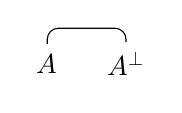
\begin{tikzpicture}
    \node (a) {$A$};
    \node (not a) [right of=a] {$A^\perp$};
    \draw [rounded corners] (a.north) -- ++ (0,0.2) -| (not a.north);
  \end{tikzpicture} \\
dont les conclusions sont $A$ et $A^\perp$.
\item[Lien coupure] Si $S$ est un réseau de conclusions $\Gamma, A$, et $S'$ un réseau de conclusions $A^\perp, \Gamma'$, alors (réseau à compléter)
  \begin{center}
    \begin{tikzpicture}
      \draw [rounded corners] (a.south) -- ++ (0,-0.2) -| (not a.south);
    \end{tikzpicture}
  \end{center}
  est un réseau de preuve de conclusions $\Gamma, \Gamma'$.
\item[Lien tenseur] Si $S$ et $S'$ sont deux réseaux de preuve de conclusions respectives $\Gamma, A$ et $B, \Gamma'$, alors
  \begin{center}
    \begin{tikzpicture}
    \end{tikzpicture}
  \end{center}
  est un réseau de preuve de conclusions $\Gamma, A \otimes B, \Gamma'$.
\item[Lien par] Si $S$ est un réseau de preuve de conclusions $\Gamma, A, B$, alors
  \begin{center}
    \begin{tikzpicture}
    \end{tikzpicture}
  \end{center}
est un réseau de preuve de conclusions $\Gamma, A \parr B$.
\end{description}
On voit facilement que ces règles correspondent aux règles d'introduction en MLL asymétrique, d'où le théorème suivant : $\vdash_{\mathrm{MLL}} \Gamma$ ssi il existe un réseau de preuve avec pour conséquences $\Gamma$.

\paragraph{Qu'a-t-on gagné ?} Les réseaux de preuve permettent d'éliminer la \emph{bureaucratie} liée à la syntaxe.

Un exemple simple : supposons qu'on ait démontré $\vdash A, B, A', B'$. Il y a 2 façons distinctes d'en déduire $\vdash A \parr B, A' \parr B'$:
\begin{center}
  \AxiomC{$\vdash A, B, A', B'$}
  \UnaryInfC{$\vdash A \parr B, A', B'$}
  \UnaryInfC{$\vdash A \parr B, A' \parr B'$}
  \DisplayProof
  \qquad
  \AxiomC{$\vdash A, B, A', B'$}
  \UnaryInfC{$\vdash A, B, A' \parr B'$}
  \UnaryInfC{$\vdash A \parr B, A' \parr B'$}
  \DisplayProof
\end{center}
Mais moralement, ces deux preuves sont les mêmes ! La présentation en \enquote{calcul des séquents}, où on doit introduire séquentiellement chaque connecteur, nous force à faire des distinctions sans pertinence. Les deux preuves ci-dessus sont identifiées à un seul réseau de preuve.

Dessin.

\paragraph{Quelles nouvelles difficultés ?} On voudrait s'assurer de la validité des réseaux de preuve. En effet, un hypergraphe étiqueté par des formules n'est pas forcément issu des règles inductives de construction, rien ne garantit a priori qu'il constitue une preuve correcte. Voici un exemple de réseau qui a l'air \emph{localement} bon, mais qui ne l'est pas :
\[ A \otimes B, A^\perp \otimes B^\perp \]
Il faut donc un critère \emph{global} pour distinguer les faux réseaux, qu'on nommera \emph{structures de preuve}, des vrais. (Contraster avec la déduction naturelle, qui n'a besoin que de vérifications locale\ldots)


\subsubsection{Réseaux de preuve pour MELL}

Dessins !



\subsection{Critères de correction pour les réseaux de preuve}


\subsubsection{Premier critère : \enquote{long trip}}

Ce critère apparaît dans l'article fondateur de Girard en 1987.


\subsubsection{Critère(s) de Danos--Regnier}

Les critères que nous allons voir ici reposent sur le passage des structures de preuve aux \emph{graphes appariés}.

\paragraph{Définition} Un graphe apparié est un triplet $(V, E, C)$ où $(V,E)$ est un graphe et $C \subseteq E \times E$ est un ensemble de paires d'arêtes. On impose que :
\begin{itemize}
\item deux arêtes appariées partagent au moins 1 sommet
\item les paries sont disjointes, i.e. chaque arête fait partie d'au plus une paire
\end{itemize}
Notation graphique : dessin

\paragraph{Conversion des structures de preuve} Soit $S$ une structure de preuve. On définit $GA(S)$ par la traduction

dessins

L'appariement n'apparaît que pour un lien $\parr$.

Ainsi, la coupure entre un tenseur et un par devient :

On définit aussi l'ensemble des \emph{graphes de correction}, $GC(S)$, comme l'ensemble des graphes obtenus en enlevant une arête de chaque paire.

Sur l'exemple ci-dessus, on obtient :

dessin

\paragraph{Critère ACC} Une structure de preuve $S$ est un réseau de preuve si et seulement si tous les graphes de correction sont acycliques et connexes.

C'est exponentiel en le nombre de liens $\parr$, ce qui est déjà mieux que le long trip qui était exponentiel en le nombre de $\parr$ et de $\otimes$.

\paragraph{Contractibilité} On peut améliorer le critère précédent en remarquant qu'on peut effectuer les opérations de contraction suivantes sur des graphes appariés sans affecter l'acyclicité ou la connexité (après retrait d'une arête de chaque paire).

dessins

Une structure de preuve $S$ est un réseau de preuve ssi, en itérant les opérations (1) et (2), on aboutit sur un unique noeud sans qu'il reste d'arête. (Attention : si on tombe sur un noeud seul avec une arête qui boucle, ce n'est pas un réseau de preuve !)

Ce critère a une très bonne performance : à chaque itération, on supprime une arête, donc on voit bien qu'on peut exécuter ça en temps polynomial, et même en $O(n^2)$ (ce n'est pas tout à fait $O(n)$ car il faut aller chercher le rédex à chaque contraction). En pratique, il est possible d'implémenter ce critère en étant très proche du temps linéaire.

\paragraph{Preuve des critères} Notre schéma de preuve sera
\begin{enumerate}
\item Réseau de preuve $\Rightarrow$ contractile
\item Contractile $\Rightarrow$ ACC
\item ACC $\Rightarrow$ réseau : c'est le plus dur
\end{enumerate}

(1) se prouve par induction structurelle sur le réseau de preuve.
\begin{itemize}
\item Le cas de base est le lien axiome : OK (dessins !)
\item Cas $\otimes$ : blah
\item Cas cut : c'est quasiment le même
\item Cas $\parr$ : blah
\end{itemize}

Pour prouver (2), on dispose d'une suite de contractions qui aboutissent sur le graphe réduit à un noeud sans boucle, qui vérifie ACC. Il suffit de montrer que ACC est préservée par antiréduction.
\begin{itemize}
\item cas des arêtes appariées entre 2 même sommets : la transformation ne change pas les graphes de correction car on enlève une des deux arêtes appariées
\item cas arête $\to$ sommet : il est clair que la connexité est préservée. S'il y a un cycle dans le graphe original, en contractant une arête, ce cycle en restera un. (Les boucles comptent comme des cycles.) Par contraposition, si le graphe contracté est acyclique, l'original le sera aussi. De même, la connexité est préservée.
\end{itemize}

Pour prouver (3), on a besoin du lemme suivant, démontré après :

\paragraph{Lemme de paire split} Soit une paire $x_1 -- b -- x_2$ dans un graphe apparié. Si, dans le graphe privé de la paire, $b$ est déconnecté de $x_1$ et $x_2$, la paire est dite \emph{paire split}.

\textbf{Lemme} : Considérons un graphe apparié \emph{fini} satisfaisant ACC. S'il contient au moins une paire, alors il contient au moins une paire split.

L'intérêt des paires split, c'est que les enlever préserve ACC.

\paragraph{Preuve de ACC $\Rightarrow$ réseau de preuve} La preuve va procéder par induction.

Dans cette induction, il faudra gérer des morceaux de structure de preuve avec des hypothèses en entrée. Donc, ce qu'on va en fait montrer, c'est : si $S$ est une structure de preuve \emph{avec hypothèses} qui satisfait le critère ACC, alors $S$ est un réseau de preuve avec hypothèses.

La récurrence procède d'abord sur le nombre de liens $\parr$ :
\begin{itemize}
\item Cas de base : $\#(\parr) = 0$
  On refait une récurrence, cette fois-ci sur le nombre de liens $\otimes$.
  \begin{itemize}
  \item cas de base : $\#(\otimes) = 0$. On n'a ni $\parr$, ni $\otimes$, et la structure de preuve doit être acyclique et connexe. Les seules possibilités sont des enchaînements d'axiome et coupure avec une même formule $A$, avec éventuellement $A$ attendu en hypothèse. Ce sont des réseaux de preuve valides.
  \item Cas inductif : $\#(\otimes) > 0$. blah
  \end{itemize}
\item Cas inductif : $\#(\parr) > 0$. On utilise le lemme paire split ici.
\end{itemize}

\paragraph{Démonstration du lemme paire split}

cf. le linear logic primer. C'est tordu et il y a plein de définitions.


\subsubsection{Graph parsing}

C'est un critère issu de l'école italienne, dû à Guerrini, Masini et Martini. Il se base sur des règles de réécriture opérant directement sur les structures de preuve.

Liste des règles (dessins).

Comme on voit, c'est extrêmement intuitif.

\paragraph{Théorème} Si la réduction aboutit sur $(NET) -- \Gamma$ alors le réseau de preuve est valide et prouve $\Gamma$.

Malgré la simplicité du critère, la preuve est compliquée.

Ce critère s'étend aux réseaux MELL, en gérant simplement les contractions, dérélictions et promotions comme suit :

dessins

Avec l'affaiblissement, il y a un souci : un réseau avec un affaiblissement n'est pas connexe. Astuce italienne : on peut faire remonter les affaiblissements dans les preuves jusqu'aux axiomes. On rajoute alors un axiome avec affaiblissement. Ca impose de rattacher l'affaiblissement à un axiome choisi arbitrairement.

\subsection{Pour aller plus loin}

\subsubsection{Géométrie de l'interaction}

\subsubsection{Réduction optimale}


\section{Les réseaux de preuve du point de vue calculatoire}

\newcommand{\lambdas}{{\lambda \mathtt{s}}}
\newcommand{\lambdalxr}{{\lambda \mathtt{l x r}}}

Dans cette partie :
\begin{itemize}
\item on voit comment se servir des réseaux de preuve pour calculer, c'est-à-dire éliminer les coupures
\item on regarde des traductions de la logique intuitionniste dans la logique linéaire qui préservent le contenu calculatoire des preuves, i.e. une traduction du $\lambda$-calcul dans les réseaux de preuve \enquote{compatible} avec les réductions
\end{itemize}

En fait, on va passer par des langages intermédiaires, qui seront des $\lambda$-calculs à substitutions explicites.

\subsection{Réduction des réseaux de preuve}

\subsubsection{Élimination des coupures en MLL}

Dessins !

En résumé :
\begin{itemize}
\item axiome + coupure $\to$ rien (Girard : l'identité est une rallonge)
\item coupure entre $A \otimes B$ et $B^\perp \parr A^\perp$ : convertie en 2 coupures ; ça fait augmenter le nombre de liens cut mais ils portent sur des formules plus petites, donc ça termine
\end{itemize}

Ces réductions préservent les long trips : dessins. Donc, si le réseau de preuve de départ était valide, on obtient toujours une preuve valide des mêmes conclusions à la fin. D'où l'utilité des critères théoriques de correction.

\subsubsection{Élimination des coupures avec les exponentielles}

Il faut rajouter des règles pour éliminer des coupures entre $\ofcourse A$ et $\whynot A^\perp$. La seule façon d'introduire un $\ofcourse$ est la boîte de promotion ; par contre, l'introduction d'un $\whynot$ peut être due à une contraction, un affaiblissement, ou une déréliction. On a droit à une règle pour chaque combinaison.

\subsubsection{Règles supplémentaires de manipulation des exponentielles}

On voit ici des règles qui ne font pas intervenir la règle cut, mais servent de la même façon à simplifier les preuves.

\subsection{Plongement de $\lambda$-calculs dans les réseaux de preuve : le $\lambdas$-calcul}

En $\lambda$-calcul, la règle $\beta$ est donnée par une opération de méta-substitution extérieure au langage : $(\lambda x.\,t)\, u \to t\{x / u \}$.

On a notamment $(u\,v)\{x/w\} = u\{x/w\}\,v\{x/w\}$ : la substitution est distribuée dans les sous-termes. Mais ceci va à l'encontre de la vision capitaliste de la logique linéaire : on a dupliqué, peut-être inutilement, une ressource.

En $\lambda \mathtt{s}$-calcul, on donnera aux substitutions un statut de première classe dans le langage. Une substitution explicite sera notée $t[x/u]$. Intuition : un $\lambdas$-terme à substitution, c'est comme un réseau de preuve avec un lien coupure.

Grammaire des termes de $\lambdas$ :

En plus de l'équivalence à $\alpha$-renommage près, on ajoute une congruence pour faire commuter les substitutions indépendantes. Quant aux règles de réduction (évidemment compatibles avec la congruence), on a :
\begin{itemize}
\item La règle $B$ : $(\lambda x.\,t)\, u \to t[x/u]$.
\item Les règles \texttt{s} : elles permettent de manipuler les substitutions, en faisant attention à ne pas distribuer inutilement sur une application.
\item Le passage au contexte.
\end{itemize}

Le système \texttt{s} est terminant et confluent, tout terme a donc une unique forme normale ; fait, il est possible de définir inductivement une fonction qui la donne (exercice). Parmi les $\lambdas$-termes, les \texttt{s}-formes normales sont exactement les termes purs, i.e. les $\lambda$-termes sans substitutions explicites

Passons maintenant à quelques propriétés intéressantes de $\lambdas$. (Preuves à compléter plus tard.)

(Ajouter purification ? c'est dans les slides)

\paragraph{Full composition} $t[x/u] \rightarrow_s^* t\{x/u\}$ pour tous termes $t$ et $u$, y compris pour $t$ non pur.

Les règles essentielles pour avoir cette propriété sont les règles de composition (\texttt{Comp1} et \texttt{Comp2}).

\paragraph{Simulation} Les réductions des termes purs existant en $\lambdas$-calcul peuvent être répercutées en $\lambda$-calcul. Autrement dit, si $t$ est un terme pur et $t \rightarrow_\beta t'$, alors $t \rightarrow_\lambdas^* t'$.

La démonstration passe par le lemme suivant : si $t \rightarrow_\lambdas t'$, alors $\mathtt{s}(t) \rightarrow_\beta^* \mathtt{s}(t')$ (où $\mathtt{s}(t)$ est la purification de $t$). Ce lemme peut être prouvé par une induction faisant intervenir une longue disjonction de cas ; illustrons quelques exemples.

\paragraph{Confluence} Le $\lambdas$-calcul est confluent.

\enquote{Diagramme commutatif} de la preuve.

Notons qu'on utilise le théorème de simulation.

\paragraph{PSN} ou \enquote{preservation of strong normalisation} : tout $\lambda$-terme fortement normalisant en $\lambda$-calcul l'est aussi en $\lambdas$.

Ce n'est pas vrai pour $\lambda \sigma$ par exemple (un contre-exemple a été trouvé par P. A. Mélliès (référence ?)).

Un exemple de calcul à substitutions explicites très simple, où on perd PSN, est $\lambda \mathrm{x}$. Dans ce langage, on ne fait pas assez attention à distribuer les substitutions uniquement quand c'est pertinent. A partir de la règle de composition, on va pouvoir construire un terme qui, en se réduisant, construit des substitutions imbriquées de plus en plus profondément : recopier l'exemple depuis les slides.



\subsection{$\lambda$-calcul vers réseaux de preuve, la suite : le $\lambdalxr$-calcul}



\end{document}
